\subsection*{Utility}

The FAB token is designed as a utility token that primarily serves as an investment vehicle and purchasing power for Fabrikator projects. Unlike traditional utility tokens, FAB is not used for platform fees, governance, or AI service payments.

\subsection*{User Tiers and Data Monetization}

Fabrikator offers two user tiers: Free and Premium.

\begin{itemize}[leftmargin=*]
    \item \textbf{Free Users:} Do not pay platform fees. Their project data may be sold by the platform (for FAB tokens) to AI trainers, creating ongoing demand for FAB. Free users pay for AI services in FIAT or TAO and can purchase marketplace content with FIAT or FAB.
    \item \textbf{Premium Users:} Pay a monthly subscription fee in FIAT for enhanced privacy; their project data is neither sold nor used for AI training. Premium users can also purchase marketplace content with FIAT or FAB. Premium users can decide to sell their projects data to earn FAB tokens when their data is used.
\end{itemize}

\subsection*{Token Utility}
\begin{itemize}[leftmargin=*]
    \item \textbf{Project Investment \& Purchasing Power:} FAB tokens provide investors with purchasing power for projects created on the platform, enabling them to acquire projects that can be used to train their AI models
    \item \textbf{Project Monetization:} Premium users can sell their completed projects for FAB tokens
    \item \textbf{Bounty Payments:} FAB tokens can be used to pay for bounties on the platform
    \item \textbf{Professional Services:} Assembly and 3D printing professionals can accept FAB as payment for their services
    \item \textbf{Data Purchases:} AI trainers and providers can purchase project data (from the platform or from premium users) using FAB tokens, creating ongoing demand. \textbf{All FAB earned from data sales is burned by the platform.}
\end{itemize}

\subsection*{Token Distribution}
\begin{itemize}[leftmargin=*]
    \item \textbf{Investors:} 40\% - For project investment and purchasing power
    \item \textbf{Team \& Development:} 20\% - Vesting over 3 years
    \item \textbf{Ecosystem Growth:} 20\% - For platform development and community incentives
    \item \textbf{Liquidity Pool:} 20\% - For FAB/TAO liquidity
\end{itemize}

\subsection*{Payment Model}
\begin{itemize}[leftmargin=*]
    \item \textbf{FAB Token:}
    \begin{itemize}
        \item Used to purchase project data (from the platform or from premium users), marketplace content, and professional services.
        \item Demand is created by AI trainers and marketplace participants.
        \item 20\% of FIAT income from premium subscriptions is used to buy and burn FAB, creating a deflationary mechanic.
    \end{itemize}
    \item \textbf{TAO (Bittensor's native token):}
    \begin{itemize}
        \item Used for all AI-related services, including model training and inference.
    \end{itemize}
    \item \textbf{FIAT Currency:}
    \begin{itemize}
        \item Used for premium subscriptions, AI services, and marketplace purchases.
        \item 20\% of premium subscription income is used to buy and burn FAB.
    \end{itemize}
    \item \textbf{Liquidity:}
    \begin{itemize}
        \item Liquidity is provided for FAB/TAO trading pairs to ensure smooth conversion between tokens and to support a healthy marketplace.
    \end{itemize}
    \item \textbf{Marketplace Fees:}
    \begin{itemize}
        \item All marketplace transactions incur a 15\% platform fee if they are performed in FIAT.
        \item All marketplace transactions incur a 5\% platform fee if they are performed in FAB. \textbf{This 5\% fee is used to burn FAB, creating additional deflationary pressure.}
    \end{itemize}
\end{itemize}

\subsection*{Token Economics}
\begin{itemize}[leftmargin=*]
    \item Total Supply: 100,000,000 FAB
    \item Raising 20,000 TAO (approximately \$8,770,000 at \$438.50 per TAO)
\end{itemize}

\subsection*{Deflationary Mechanism}

To ensure long-term value and scarcity, 20\% of all FIAT income from premium subscriptions is used by the platform to purchase FAB tokens on the open market, which are then permanently burned. Additionally, the 5\% fee collected from all marketplace transactions performed in FAB is also burned, and all FAB earned from data sales to AI trainers is burned, further increasing the deflationary effect and buy pressure on FAB.

\subsection*{Use of Funds}
The funds raised and generated through the Fabrikator platform are allocated as follows:
\begin{itemize}[leftmargin=*]
    \item \textbf{20\%} of premium subscription FIAT income is used to buy and burn FAB tokens.
    \item \textbf{80\%} of premium subscription FIAT income goes to the treasury for platform maintenance, scaling, AI model training, and potential buyouts of successful marketplace models.
    \item \textbf{Marketplace Fees:} 5-15\% platform fee is taken from all marketplace transactions.
    \item \textbf{Other allocations:} Funds may also be used for marketing, community growth, and ecosystem partnerships as needed.
\end{itemize}

These allocations are designed to maximize platform growth, user adoption, and long-term sustainability.

% --- Improved Projected Income Section ---

\subsection*{Projected Income}

To illustrate the platform's earning potential and the resulting FAB buy and burn pressure, we project monthly income and FAB demand as the user base grows from 1 to 20,000 users. The following assumptions are used:

\begin{itemize}[leftmargin=*]
    \item 1 in 7 users is a premium user (\textasciitilde14.3\%), 6 in 7 are free users.
    \item Premium monthly fee: \$150.
    \item All users spend \$50/month on AI usage (platform takes 15\% fee).
    \item All users spend \$20/month on the marketplace in FIAT (15\% fee) and \$5/month in FAB (5\% fee, \textbf{all of which is burned}).
    \item 20\% of premium FIAT income is used to buy and burn FAB.
    \item \textbf{AI trainers purchase data for \$1/month in FAB per free user} (\textasciitilde6/7 of total users), \textbf{all of which is burned by the platform}.
\end{itemize}

\textbf{Formulas:}

\begin{itemize}[leftmargin=*]
    \item Premium users: $N_{\text{premium}} = \frac{N_{\text{total}}}{7}$
    \item Free users: $N_{\text{free}} = N_{\text{total}} \times \frac{6}{7}$
    \item FIAT income from premiums: $I_{\text{premium}} = N_{\text{premium}} \times 150$
    \item AI usage fee income: $I_{\text{AI}} = N_{\text{total}} \times 50 \times 0.15$
    \item Marketplace FIAT fee: $I_{\text{mkt,FIAT}} = N_{\text{total}} \times 20 \times 0.15$
    \item Marketplace FAB fee (burned): $I_{\text{mkt,FAB}} = N_{\text{total}} \times 5 \times 0.05$
    \item \textbf{Total FIAT income:} $I_{\text{FIAT,tot}} = I_{\text{premium}} + I_{\text{AI}} + I_{\text{mkt,FIAT}}$
    \item \textbf{FIAT used to buy and burn FAB:} $B_{\text{FAB,FIAT}} = I_{\text{premium}} \times 0.2$
    \item \textbf{FAB burned (marketplace + data):} $B_{\text{FAB,direct}} = I_{\text{mkt,FAB}} + N_{\text{free}}$
    \item \textbf{Total FAB burned:} $B_{\text{FAB,tot}} = B_{\text{FAB,FIAT}} + B_{\text{FAB,direct}}$
\end{itemize}

\begin{center}
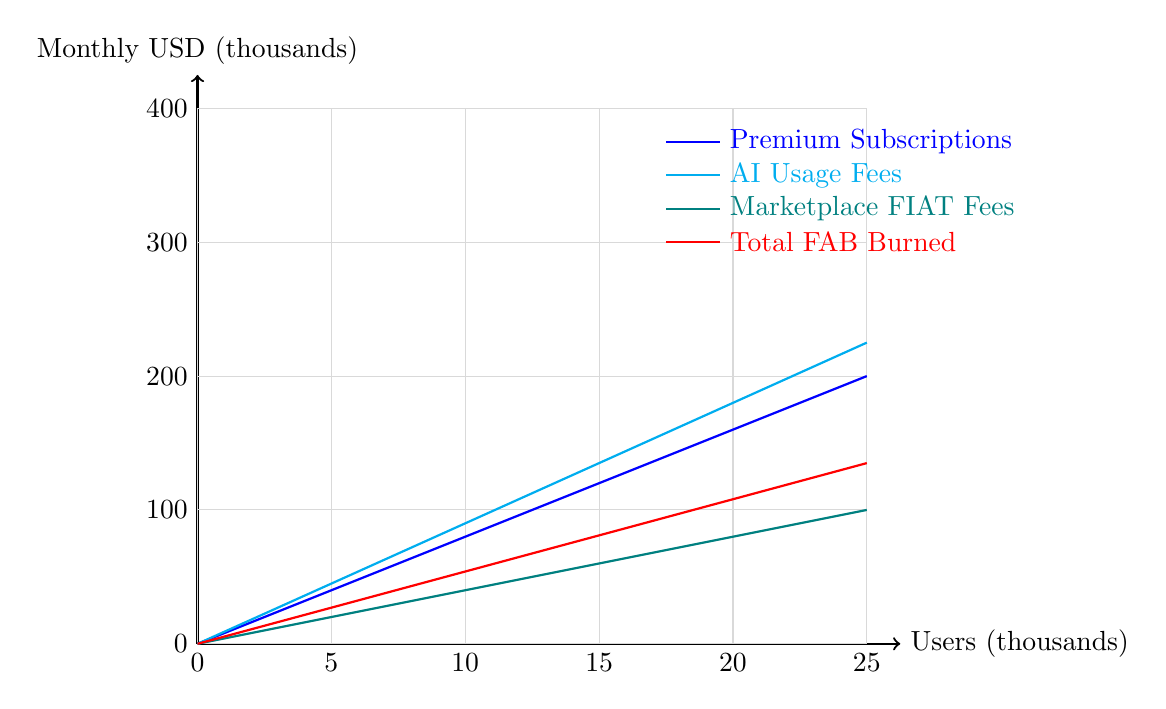
\begin{tikzpicture}[scale=0.85]
    % Define the axes
    \draw[thick, ->] (0,0) -- (10.5,0) node[right] {Users (thousands)};
    \draw[thick, ->] (0,0) -- (0,8.5) node[above] {Monthly USD (thousands)};
    
    % Draw grid
    \foreach \x in {0,2,...,10}
        \draw[gray!30] (\x,0) -- (\x,8);
    \foreach \y in {0,2,...,8}
        \draw[gray!30] (0,\y) -- (10,\y);
    
    % X-axis labels
    \foreach \x/\label in {0/0, 2/5, 4/10, 6/15, 8/20, 10/25}
        \node[below] at (\x,0) {\label};
    
    % Y-axis labels
    \foreach \y/\label in {0/0, 2/100, 4/200, 6/300, 8/400}
        \node[left] at (0,\y) {\label};
    
    % Plot FIAT income from premium subscriptions
    \draw[blue, thick] plot coordinates {
        (0,0) (2,0.8) (4,1.6) (6,2.4) (8,3.2) (10,4.0)
    };
    
    % Plot FIAT income from AI usage fees
    \draw[cyan, thick] plot coordinates {
        (0,0) (2,0.9) (4,1.8) (6,2.7) (8,3.6) (10,4.5)
    };
    
    % Plot FIAT income from marketplace fees
    \draw[teal, thick] plot coordinates {
        (0,0) (2,0.4) (4,0.8) (6,1.2) (8,1.6) (10,2.0)
    };
    
    % Plot Corrected Total FAB burning (with correct calculation)
    \draw[red, thick] plot coordinates {
        (0,0) (2,0.54) (4,1.08) (6,1.62) (8,2.16) (10,2.7)
    };
    
    % Legend
    \draw[blue, thick] (7,7.5) -- (7.8,7.5) node[right] {Premium Subscriptions};
    \draw[cyan, thick] (7,7.0) -- (7.8,7.0) node[right] {AI Usage Fees};
    \draw[teal, thick] (7,6.5) -- (7.8,6.5) node[right] {Marketplace FIAT Fees};
    \draw[red, thick] (7,6.0) -- (7.8,6.0) node[right] {Total FAB Burned};
\end{tikzpicture}
\end{center}

% Key points from table
\begin{center}
\begin{tabular}{|c|c|c|c|c|}
\hline
\textbf{Users} & \textbf{Premium Users} & \textbf{Free Users} & \textbf{Monthly FIAT} & \textbf{Monthly FAB Burned} \\
\hline
1,000 & 143 & 857 & \$21,428 & \$5,397 \\
5,000 & 714 & 4,286 & \$107,143 & \$26,956 \\
10,000 & 1,429 & 8,571 & \$214,286 & \$53,941 \\
25,000 & 3,571 & 21,429 & \$535,714 & \$134,815 \\
\hline
\end{tabular}
\end{center}

\textbf{Notes:}
\begin{itemize}[leftmargin=*]
    \item \textbf{Total FIAT Income} includes premium subscriptions, AI usage fees, and marketplace FIAT fees.
    \item \textbf{FIAT Used to Buy \& Burn FAB} is the amount of FIAT from premium subscriptions used monthly to buy and burn FAB (20\%).
    \item \textbf{FAB Burned (Marketplace + Data)} includes the 5\% fee on marketplace FAB transactions plus the \$1 per free user from data sales.
    \item \textbf{Monthly FAB Burned} is the total of all FAB burning mechanisms combined.
    \item At 20,000 users, approximately \$108,000 worth of FAB is burned monthly.
\end{itemize} 